As part of our installation, we have two modes of putting the image on your Raspberry Pi. These are tailored to users who just want an express installation with no difficulties, and for users who wish to build their own Pilight image from scratch using the Yocto Builder.
\subsection{Express install}
The wiki on Github has a link to a prebuilt image of the Pilight system we had in place at expo. This image is updated using Yocto's autobuilder program Toaster. Once downloaded, it can be installed like any other image for a Raspberry Pi.
\subsubsection{Windows}
Windows will use the graphical utility Win32DiskImager to install our image to the SD card.
\begin{itemize}
   \item Download the image from the Pilight Wiki at \url{https://github.com/rettigs/cs-senior-capstone/wiki}
   \item Insert the SD card into your SD card reader and check which drive letter was assigned. You can easily see the drive letter, such as G:, by looking in the left column of Windows Explorer. You can use the SD card slot if you have one, or a cheap SD adapter in a USB port.
   \item Download the Win32DiskImager program from \url{http://sourceforge.net/projects/win32diskimager/}, which will provide a way to put the image on the SD card
   \item Extract the executable from the zip file and run the Win32DiskImager utility; you may need to run this as administrator. Right-click on the file, and select Run as administrator.
   \item Select the image file you extracted earlier.
   \item Select the drive letter of the SD card in the device box. Be careful to select the correct drive; if you get the wrong one you can destroy the data on your computer's hard disk! If you are using an SD card slot in your computer and can't see the drive in the Win32DiskImager window, try using an external SD adapter.
   \item Click Write and wait for the write to complete.
   \item Exit the imager and eject the SD card.
\end{itemize}
\subsubsection{OSX}
On Macs we can use the command-line utilities for creating our image.
\begin{itemize}
   \item Insert your SD card to an SD card reader
   \item Use the disk reader program to identify your SD card:
      \begin{lstlisting}
      diskutil list
      \end{lstlisting}
   \item Identify the disk (not partition) of your SD card e.g \textit{disk4}, not \textit{disk4s1}
   \item Unmount the SD card
      \begin{lstlisting}
      diskutil unmountDisk /dev/disk<disk# from diskutil>
      \end{lstlisting}
      where \textit{disk} is your BSD name e.g. \textit{diskutil unmountDisk /dev/disk4}
   \item Copy the data to the SD card:
      \begin{lstlisting}
      sudo dd bs=1m if=pilight.img of=/dev/rdisk<disk# from diskutil>
      \end{lstlisting}
      where \textit{disk} is your BSD name e.g. \textit{/dev/disk4}
      \begin{itemize}
         \item This may result in a \textit{dd: invalid number '1m'} error if you have GNU coreutils installed. In that case, just change the \textbf{bs=1m} to \textbf{bs=1M}
      \end{itemize}
\end{itemize}
\subsubsection{Linux}
Our Linux install is similar to OSX, but using Linux tools instead
\begin{itemize}
   \item Run \textit{df} to find where your SD card is mounted:
      \begin{lstlisting}
      df -h
      \end{lstlisting}
      It will be listed as something like \textit{/dev/mmcblk0p1} or \textit{/dev/sdd1}. For later steps, you'll need the name without the partition number, which would change the values to \textit{/dev/mmcblk0} and \textit{dev/sdd}
   \item Unmount the drive. For \textit{/dev/sdd} it would be:
      \begin{lstlisting}
      umount /dev/sdd1
      \end{lstlisting}
   \item Write the data to the SD card. Again for \textit{/dev/sdd} it would be:
      \begin{lstlisting}
      dd bs=4M if=pilight.img of=/dev/sdd
      \end{lstlisting}
   \item Run sync to flush the write cache
      \begin{lstlisting}
      \end{lstlisting}
\end{itemize}
\subsection{Yocto Build}
Using the Yocto autobuilder allows you to build the image from scratch, however it does require some advanced knowledge of the Linux command line. You'll also need about 30 GB of drive space for the build.
\begin{itemize}
   \item Start by fetching the builder and all the source repositories we'll need
      \begin{lstlisting}
      mkdir source
      cd source
      git clone -b dizzy git://git.yoctoproject.org/poky
      cd poky
      git clone -b dizzy git://git.openembedded.org/meta-openembedded
      git clone -b dizzy git://git.yoctoproject.org/meta-intel-iot-middleware
      git clone -b dizzy https://github.com/Pilight/meta-pilight.git
      \end{lstlisting}
   \item Initialize the build environment
      \begin{lstlisting}
      source oe-init-build-env
      \end{lstlisting}
   \item Now add the layers to the bblayers file and the configuration options to the local.conf file:
      \begin{lstlisting}
      echo "BBLAYERS += \"$HOME/source/poky/meta-pilight\"" >> conf/bblayers.conf
      echo "BBLAYERS += \"$HOME/source/poky/meta-openembedded/meta-python\"" >> conf/bblayers.conf
      echo "BBLAYERS += \"$HOME/source/poky/meta-openembedded/meta-oe\"" >> conf/bblayers.conf
      echo "BBLAYERS += \"$HOME/source/poky/meta-openembedded/meta-networking\"" >> conf/bblayers.conf
      echo "MACHINE = \"raspberrypi2\"" >> conf/local.conf
      echo "CORE\_IMAGE\_EXTRA\_INSTALL += \"kernel-dev\"" >> conf/local.conf
      echo "CORE\_IMAGE\_EXTRA\_INSTALL += \"pilight\"" >> conf/local.conf
      echo "MACHINE\_FEATURES\_BACKFILL\_CONSIDERED += \"rtc"\" >> conf/local.conf
      echo "EXTRA\_IMAGE\_FEATURES = \"debug-tweaks package-management dev-pkgs tools-sdk dev-pkgs\"" >> conf/local.conf
      \end{lstlisting}
   \item Now build your image. This could take several hours depending on the system:
      \begin{lstlisting}
      bitbake maker-image
      \end{lstlisting}
   \item Using Yocto's builtin installer script, we can write the image to the SD card. Assuming it's at \textit{/dev/sdd}:
      \begin{lstlisting}
      sudo poky/scripts/contrib/mkefidisk.sh \
      /dev/sdd \
      poky/build/tmp/deploy/images/raspberrypi2/pilight-image-raspberrypi2.hddimg \
      /dev/sda
      \end{lstlisting}
      We now have a bootable SD card
\end{itemize}
\section{Usage}
\subsubsection{Hardware setup}
Setting up the hardware depends on how you want to use the Pilight system. If you want to control a standard light switch, for example, you'll need to replace the light switch itself. Before connecting the existing power line to the relay, cut off the power to the switch for safety. Simply connect the live wire to the relay as shown here:\\
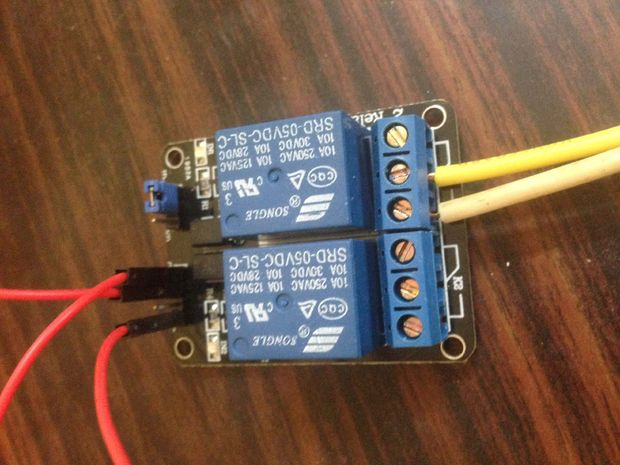
\includegraphics[scale=0.5]{relay}\\
To connect the ESP8266 module to the relay, you'll need to connect each one of the connections you want to use on the ESP module to the corresponding relay pin. For instance, connecting pin 1 on the ESP to relay in IN1 will allow you to control the light on IN1 with pin 1 on the ESP module.\\
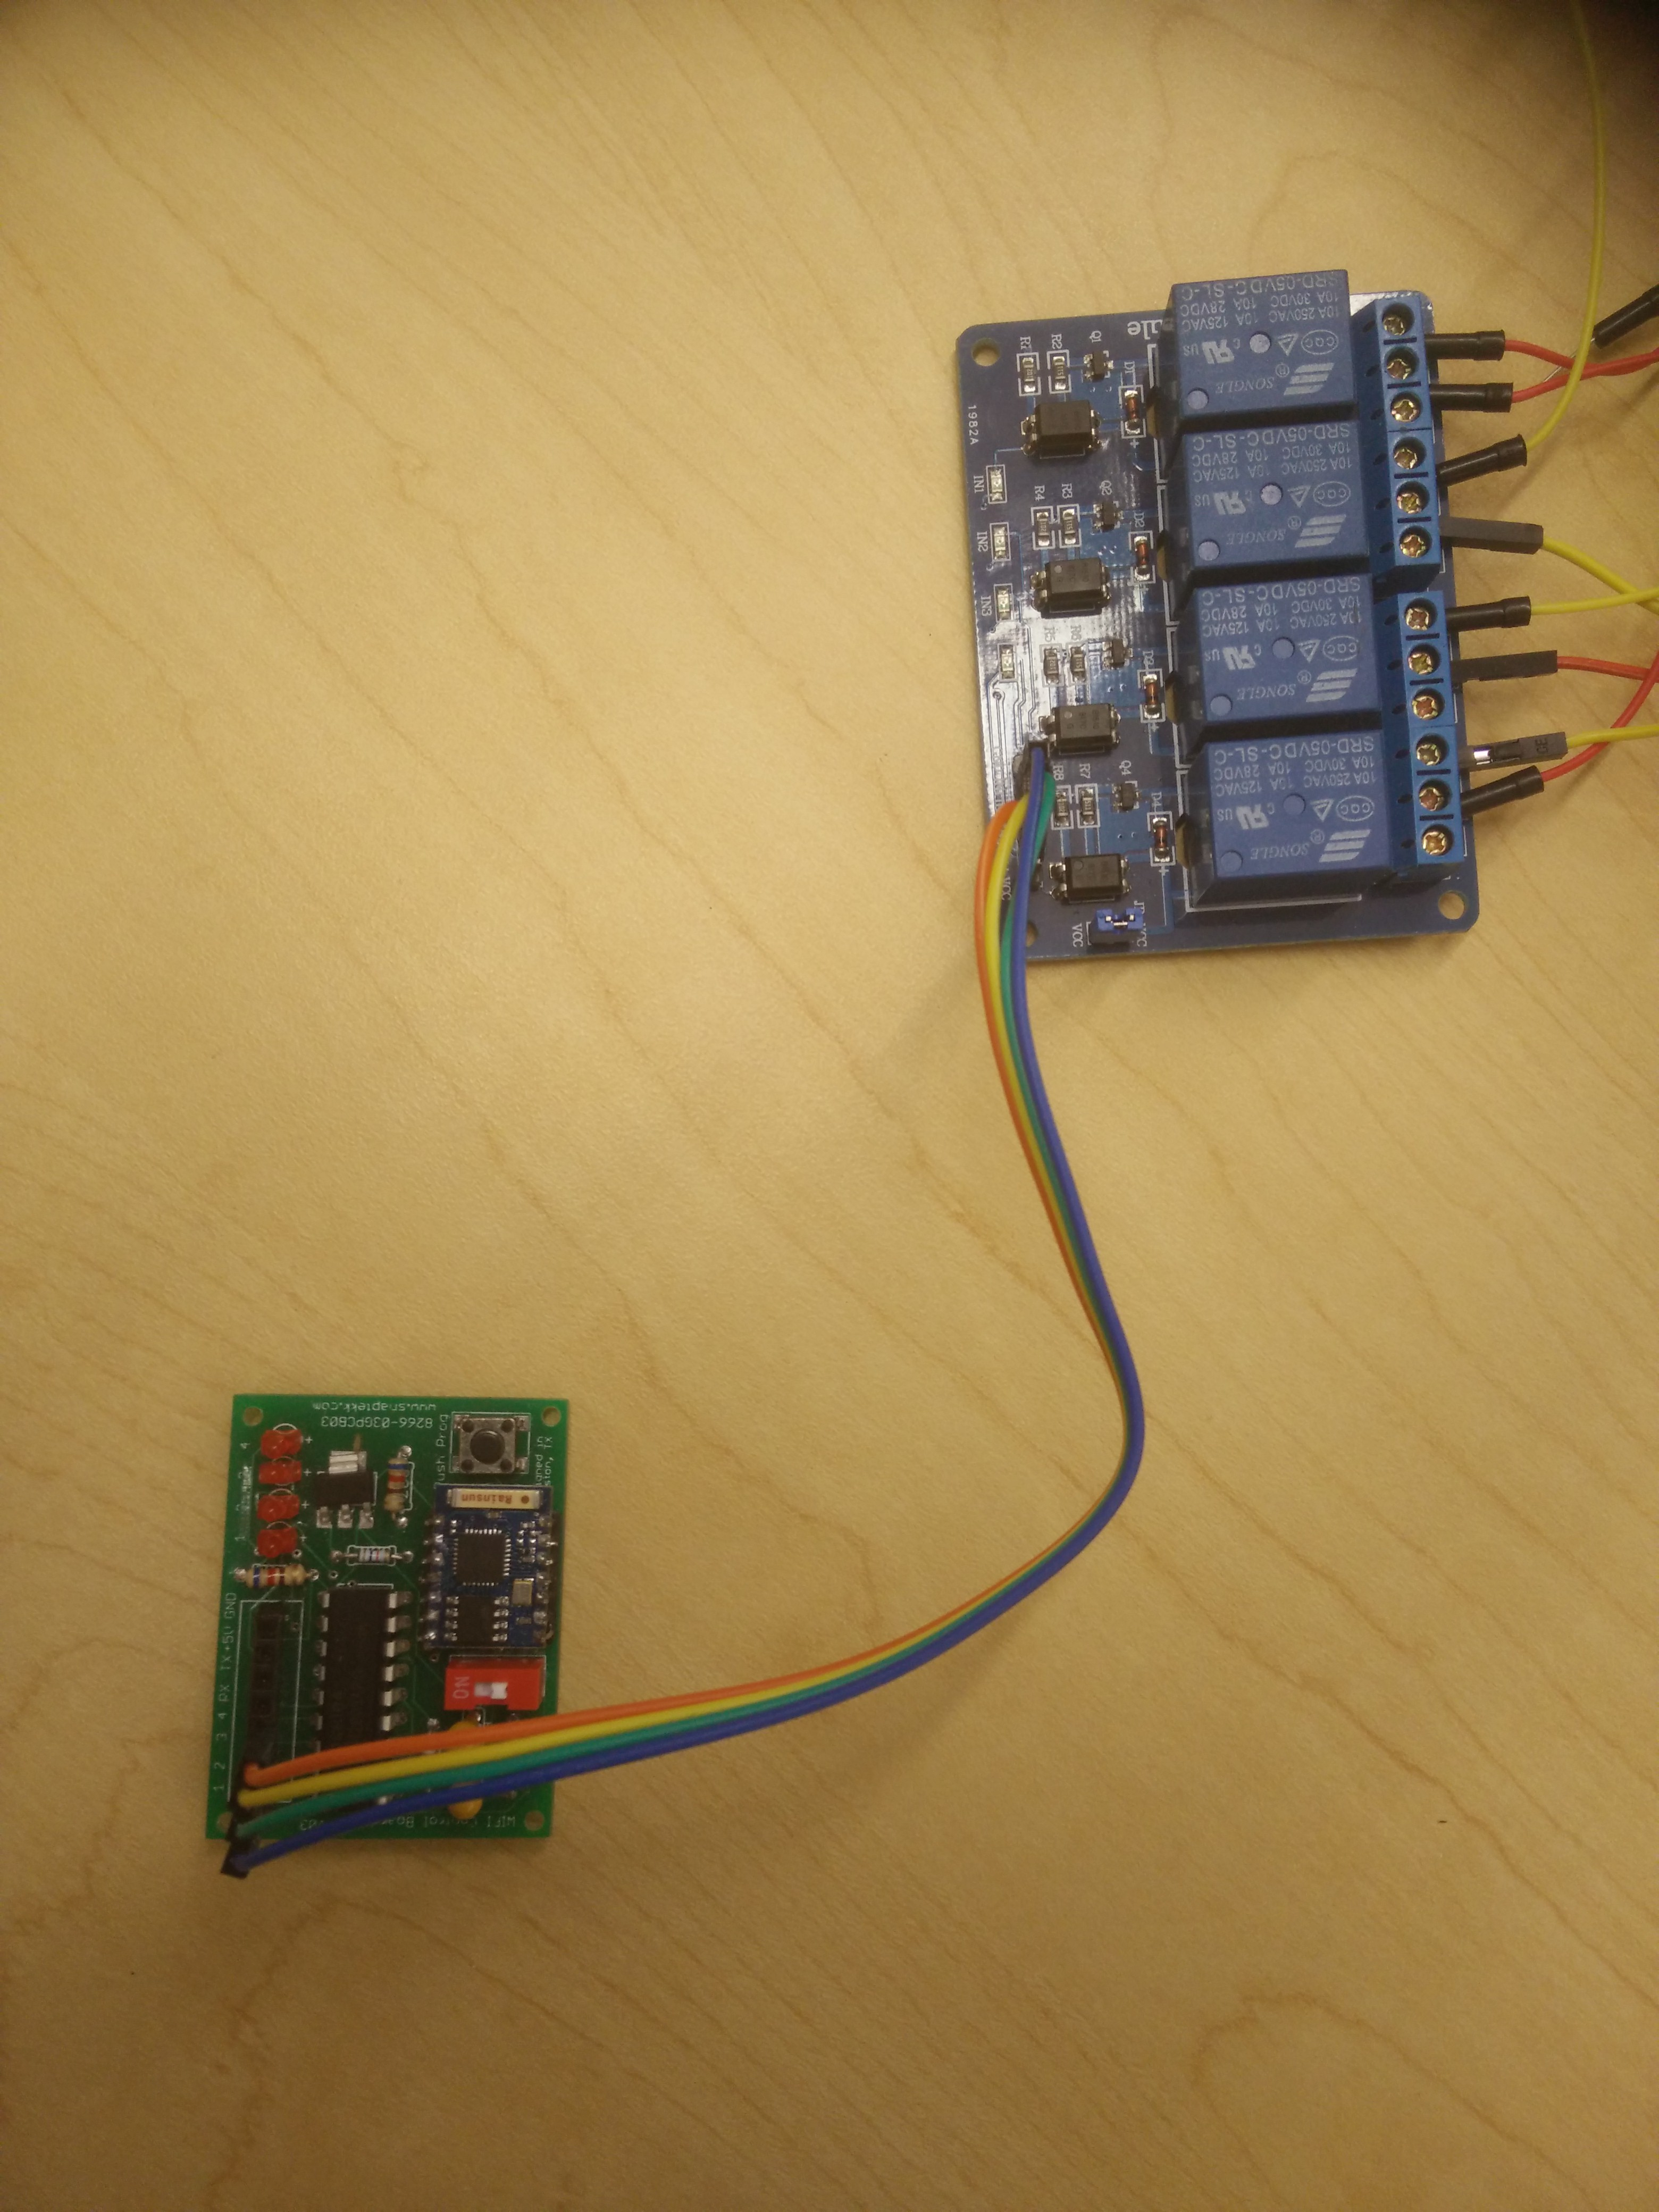
\includegraphics[scale=0.05]{connection}\\
Both the relay and the ESP module will need 5V power supplied. You can either run these through a wall outlet with a 5V power supply, or try a long-term battery. Use what works best for your electrical setup. To set up the Raspberry Pi, just provide it with standard wall power over a micro USB cable.
\subsubsection{Software Setup}
Once the system is booted on the SD card, you'll see the web interface appear on the TFT LCD screen. You can also access it by logging onto the "Pilight\_Access" wireless access point on a smartphone, tablet or computer. The default password is "RaspberryPi" for connecting. Once you're on, go to \textbf{http://192.168.42.1} in your web browser to access the interface.\\
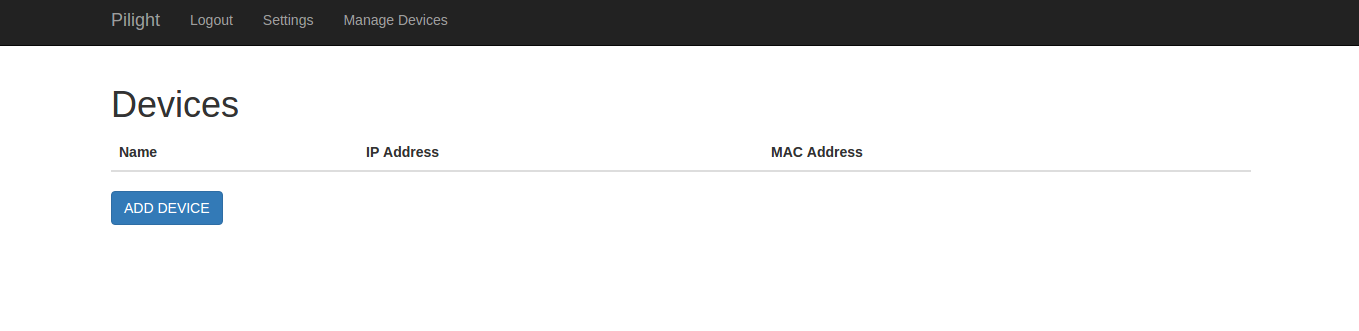
\includegraphics[width=1.0\textwidth]{devices.png}\\
Assuming the ESP8266 modules are powered on with 5v and connected up to the relay, you can add the devices on the "Manage Devices" page. Click on the "Add Devices" button to add the ESP8266 devices to the list. Once it's done checking for devices, all your modules should appear.\\
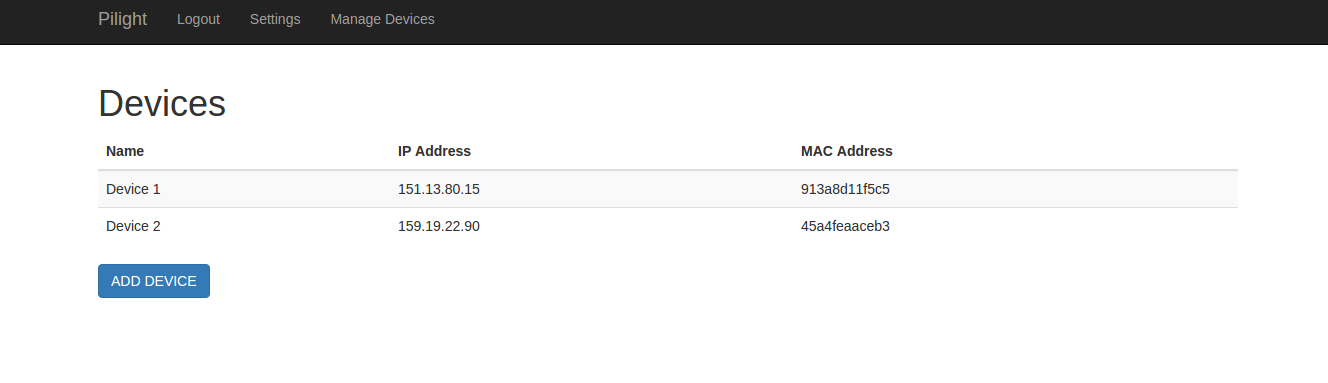
\includegraphics[width=1.0\textwidth]{added-devices.png}\\
With these devices added, the front page will automatically populate itself with listings of your new devices. The ESP8266 modules used for this project have 4 GPIOs for controlling the lights, so you'll find 4 entries per device. The front page lets you reorganize these lights into groups for control, and with it you can set intelligent rules for turning these lights on and off
\subsubsection{Controlling Lights}
To control groups of lights, you can create an empty group using the "Create Group" button at the bottom of the page. Clicking and dragging lights and groups on the movement icon on the left side of the button will allow you to create groups. You can nest groups within other groups or have lights independent of groups. Clicking the gear icon to the right of the name of a light or group will take you to the configuration page.\\
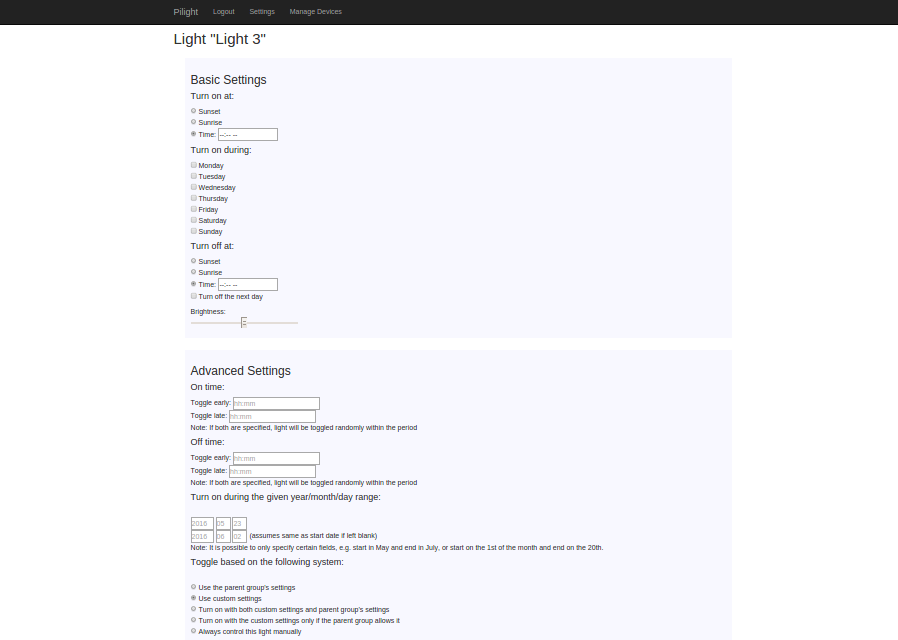
\includegraphics[width=1.0\textwidth]{advanced.png}\\
